\documentclass[12pt, a4paper]{article}
%=========================== PACKAGES =============================%

\usepackage[utf8]{inputenc}
\DeclareUnicodeCharacter{00A0}{ }

\usepackage[hmargin=1.5cm,vmargin=1.5cm]{geometry}
\usepackage[brazil]{babel}

\usepackage{longtable}

\usepackage{graphicx}
\usepackage{placeins}
\usepackage{subcaption}
\usepackage{float}

\usepackage{hhline}
\usepackage{courier}

\usepackage{amsmath}
\usepackage{bm}
\usepackage{amsfonts}

\usepackage[hyphens]{url}

\usepackage{listings}
\renewcommand\lstlistingname{Programa}


\usepackage{color} %red, green, blue, yellow, cyan, magenta, black, white
\lstset{language=bash,%
basicstyle=\footnotesize\ttfamily,
breaklines=true,%
keywordstyle=[4]{\color{black}},
frame= single,
}

\lstdefinestyle{nonumbers}
{numbers=none}

\usepackage{multirow}

\usepackage{float}

\usepackage{enumerate}

\begin{document}

%    \maketitle
{\large
\centerline{\textbf{Relatório Exercício Prático 8}}
\centerline{Gustavo Ciotto Pinton 117136}
\centerline{EA979 - Processamento de Imagens}
}

\section* {Explicação}

O modelo de iluminação proposto por Phong é composto pela soma de três
componentes, sendo elas, ambiente, difusa e especular. A iluminação
\textbf{ambiente} atinge todos os objetos em todas as direções de maneira
similar e é refletida, consequentemente, em todas elas também. A luz \textbf{difusa}, por sua vez, é
proveniente de uma fonte pontual e atinge cada objeto  \(i\) da cena com um ângulo
\(\theta_i\), que consiste no ângulo entre a normal da respectiva superfície e a
direção com que a luz atinge \(i\). Essa luz é refletida em todas as direções
com intensidades variando em função de \(\cos \theta_i\). Assim, esse tipo de
iluminação depende da posição da fonte em relação aos objetos. Por fim, a luz
\textbf{especular} também provém de uma fonte pontual, porém depende do tipo de
material com que o objeto é feito e da posição do observador. O primeiro
determina uma espécie de campo de reflexão, isto é, um intervalo de ângulos em que o
observador visualizará a luz refletida, dependendo de seu posição. Materiais
como o espelho possuem um intervalo bem pequeno de reflexão e, em oposição, objetos feitos de plástico,
por exemplo, um grande campo. Em outras palavras, tal modelo aproxima-se do
conceito de brilho, caracterizado pelos tipos de materiais.

\vspace{12pt}

Para ativar a iluminação, a biblioteca \textit{OpenGL} disponibiliza a função
\texttt{glEnable}. \textit{OpenGL} oferece suporte a várias fontes de
iluminação, porém vamos utilizar somente uma delas, identificada por
\texttt{GL\_LIGHT1}. O código utilizado para habilitar a iluminação é, portanto:

\begin{lstlisting}[keywordstyle=\ttfamily, style=nonumbers]
glEnable(GL_LIGHTING);
glEnable(GL_LIGHT1);
\end{lstlisting}

\vspace{12pt}

A atribuição das três iluminações é realizada por uma mesma função, chamada de
\path{glLightfv}, recebendo como parâmetro a identificação da fonte (neste
caso, sempre \texttt{GL\_LIGHT1}), o tipo de iluminação (ambiente, difusa ou
especular) e as características relacionadas a ela (cor ou posição, por
exemplo). As 3 figuras abaixo representam cada um dos três tipos de iluminação
utilizados \textbf{separadamente}, para um fonte luminosa posicionada no eixo
\(z\), nas coordenadas \((0, 0, 5)\), isto é, no mesmo eixo e local em que o
observador se encontra.

\FloatBarrier

\begin{figure}[h!]

\centering

\begin{subfigure}{.33\textwidth}
\centering
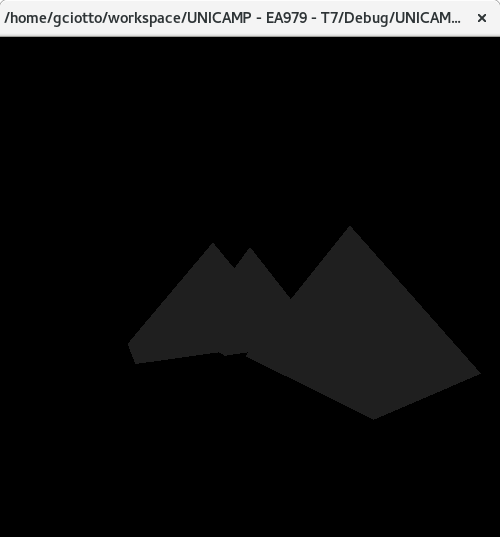
\includegraphics[scale=0.33]{ambiente}
\caption{\centering \path{GL_AMBIENT}, \(RGBA = (0.4, 0.4, 0.4, 1.0 )\)}
\label{img:ambient}
\end{subfigure}%
\begin{subfigure}{.33\textwidth}
\centering
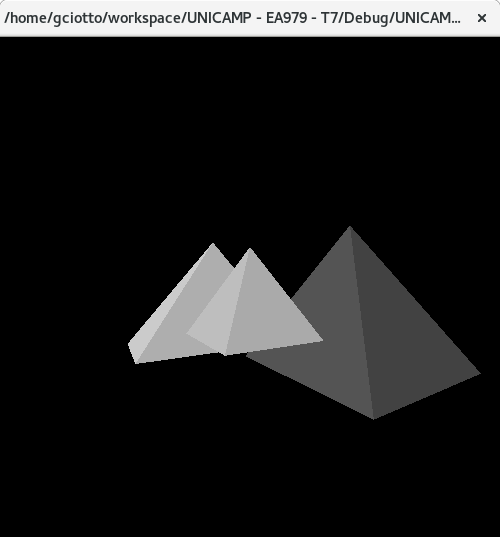
\includegraphics[scale=0.33]{difusa}
\caption{\centering \path{GL_DIFFUSE}, \(RGBA = (1.0, 1.0, 1.0, 1.0 )\)}
\label{img:diffuse}
\end{subfigure}
\begin{subfigure}{.33\textwidth}
\centering
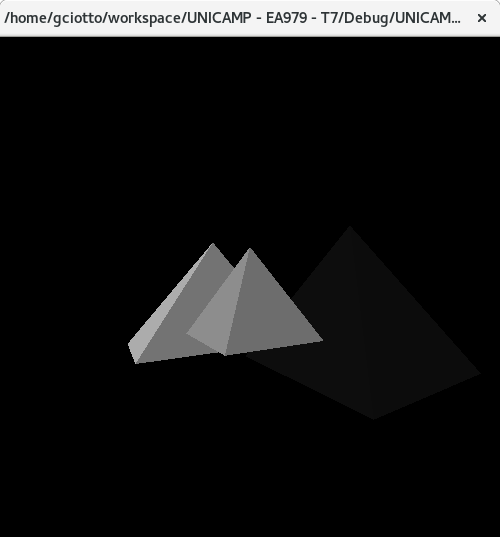
\includegraphics[scale=0.33]{especular}
\caption{\centering \path{GL_SPECULAR}, \(RGBA = (1.0, 1.0, 1.0, 1.0 )\)}
\label{img:specular}
\end{subfigure}


\caption{Tipos de ilumicação utilizados \textbf{separadamente}.}
\end{figure}

\FloatBarrier

Observa-se que 

\begin {enumerate}[i.]
  \item A iluminação ambiente, figura \ref{img:ambient}, não acrescenta a noção
  de profundidade ao objeto, uma vez que ilumina todas as faces de uma maneira
  similar.

  \item  A iluminação difusa, figura \ref{img:diffuse}, depende da posição da
  fonte. Objetos posicionados mais próximos ao eixo \(z\), isto é, pirâmides do centro e à esquerda, são
  iluminados mais fortemente. A pirâmide mais à direita, estando mais distante
  de \(z\), reflete menos luminosidade, visto que o cosseno para ângulos
  próximos de 90º é pequeno.

  \item A ilumicação especular, figura \ref{img:specular}, depende do material e
  posicões do observador e fonte. Para a especificação do material, utilizamos o
  trecho abaixo. A função \path{glMaterialfv} especifica os parâmetros do
  material para o modelo de iluminação. Em especial, o parâmetro
  \path{GL_SHININESS} especifica o expoente \(ns\) da fórmula \((\cos
  \phi)^{ns}\).
  
\begin{lstlisting}[keywordstyle=\ttfamily, style=nonumbers] 
GLfloat mat_specular[] = { 1.0, 1.0, 1.0, 1.0 };
GLfloat mat_shininess[] = { 05.0 };
glMaterialfv(GL_FRONT, GL_SPECULAR, mat_specular);
glMaterialfv(GL_FRONT, GL_SHININESS, mat_shininess);
\end{lstlisting}

\end{enumerate}


A figura abaixo representa a soma das três figuras acima.

\FloatBarrier

\begin{figure}[h!]
\centering
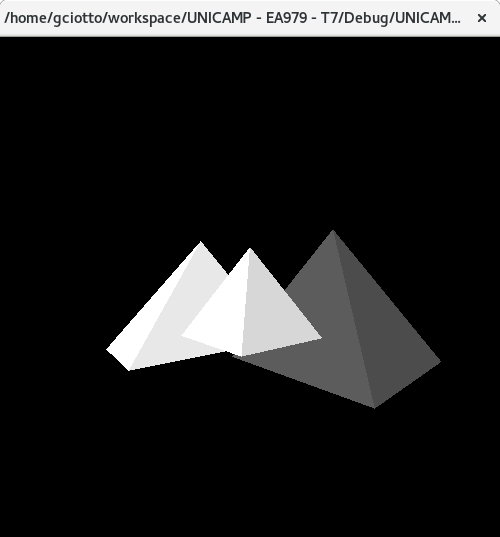
\includegraphics[scale=0.35]{total}
\caption{Renderização de 3 pirâmides com iluminação.}
\label{img:total}
\end{figure}

\FloatBarrier

As figuras abaixo foram geradas para diferentes parâmetros das iluminações. Para
a luz ambiente, utilizamos \(RGBA_{ambient} = (0.1, 0.1, 0.1, 1.0)\), para a
difusa usamos somente a componente azul, isto é, \(RGBA_{diffuse} = (0, 0,
1.0, 1.0)\), e, para a especular, diminuimos o exponente para \(ns = 2\). Além
disso, posicionamos a fonte à esquerda dos objetos, na posição \((5, 2, 0)\).


\FloatBarrier

\begin{figure}[h!]

\centering

\begin{subfigure}{.245\textwidth}
\centering
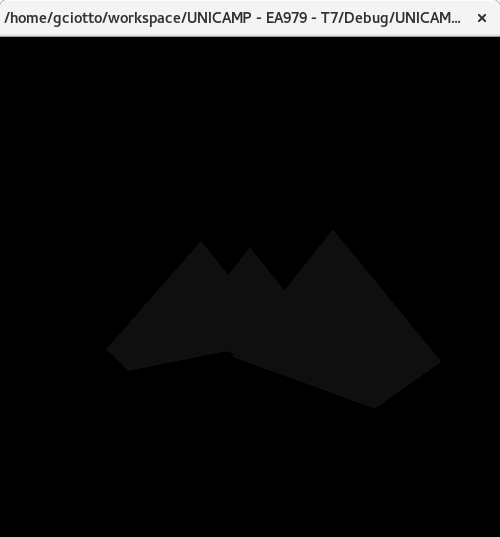
\includegraphics[scale=0.25]{ambient2}
\caption{\centering \path{GL_AMBIENT}}
\label{img:ambient2}
\end{subfigure}%
\begin{subfigure}{.245\textwidth}
\centering
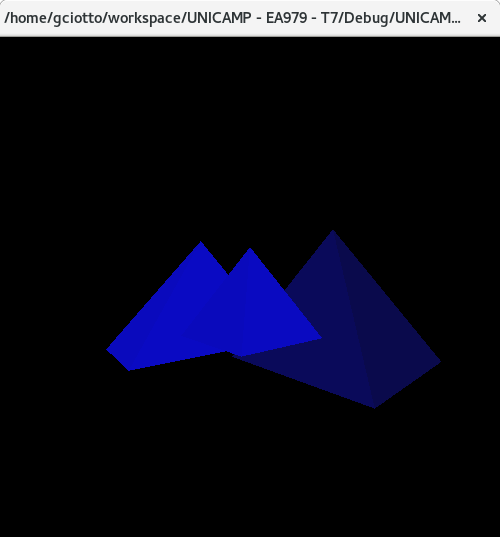
\includegraphics[scale=0.25]{diffuse2}
\caption{\centering \path{GL_DIFFUSE}}
\label{img:diffuse2}
\end{subfigure}
\begin{subfigure}{.245\textwidth}
\centering
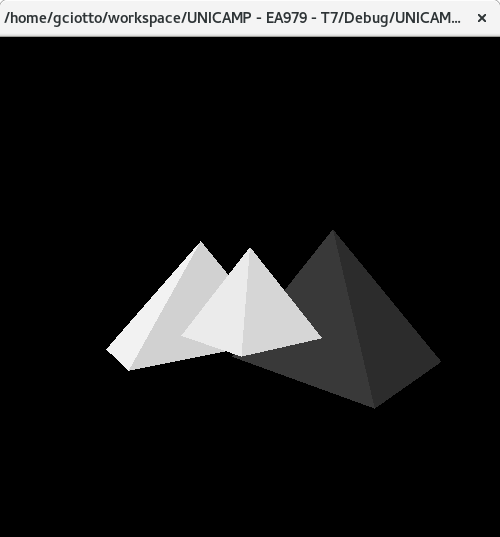
\includegraphics[scale=0.25]{specular2}
\caption{\centering \path{GL_SPECULAR}}
\label{img:specular2}
\end{subfigure}
\begin{subfigure}{.245\textwidth}
\centering
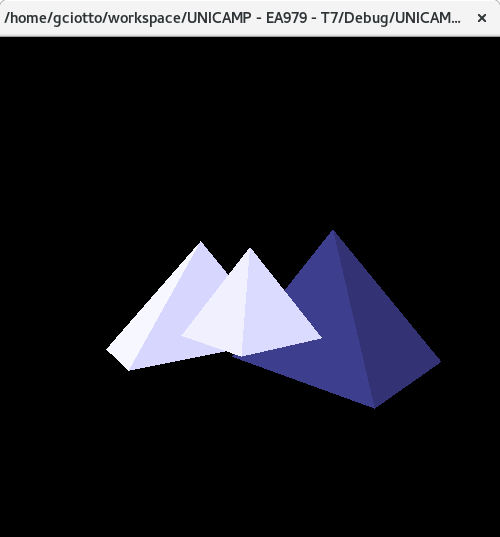
\includegraphics[scale=0.25]{todas2}
\caption{\centering Todas as iluminações.}
\label{img:all}
\end{subfigure}


\caption{Tipos de ilumicação utilizados \textbf{separadamente}.}
\end{figure}

\FloatBarrier

\section* {Referências}

\begin {enumerate}
  \item \textit{OpenGL Programming Guide Chapter 5}, disponível em
  \url{http://www.glprogramming.com/red/chapter05.html}.
\end{enumerate}

\end{document}